\begin{figure}[ht]
\centering
	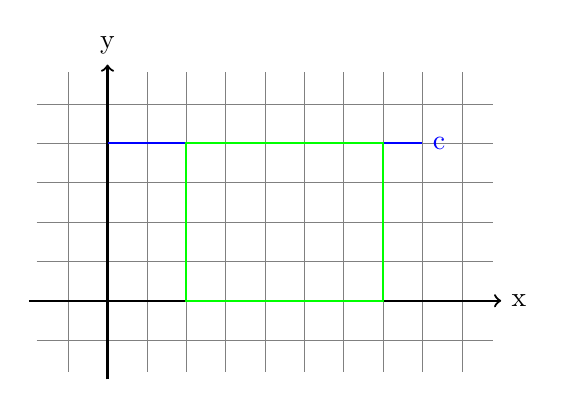
\begin{tikzpicture}
		\draw[very thin, gray, step = 0.5] (-0.9,-0.9) grid (4.9,2.9);
		\draw[->,thick, black](-1,0) -- (5,0) node[right]{x};
		\draw[->,thick, black](0,-1) -- (0,3) node[above]{y};
		\draw[thick,blue](0,2) -- (4,2) node[right]{c};
		\draw[green,thick](1,0) rectangle (3.5,2);
	\end{tikzpicture}
	\caption{Konstante Funktion}
		\label{fig_int_konst_funk}
\end{figure}